In this section, we will give brief overview of the provided data for solving our university space optimization problem. We have been provided with the following datasets:

\begin{table}[H]
\centering
\begin{tabular}{|l|l|l|}
\hline
\# & \textbf{Dataset Name} & \textbf{Dataset Description}                                           \\ \hline
1  & \texttt{uom-space}             & Space metadata of all rooms across campuses and buildings              \\ \hline
2  & \texttt{rm-category-type}      & Definition of all UoM standard room categories and types               \\ \hline
3  & \texttt{fl-name}               & Dataset to provide more information about building floors              \\ \hline
4  & \texttt{av-equipment}         & Audio Visual equipment data including its location information         \\ \hline
5  & \texttt{em-location}           & De-identified employee/staff location data                             \\ \hline
6  & \texttt{2020-timetable-v2}     & Latest class scheduling data including a class's time and its location \\ \hline
7  & \texttt{meeting-room-usage}    & Collected data of meeting room usage                                   \\ \hline
\end{tabular}
\caption{Provided datasets}
\end{table}

\subsection{Exploratory Data Analysis}

In this section, we have explored all the provided datasets to understand their properties, size, and scale. We have also performed an analysis of how these datasets correlate with the provided problem.

\subsubsection{What are the different properties, size, and scale of data?}

After importing all the provided datasets using \texttt{pandas} python package, we deduced the following summary of the data as shown in the below tables.

\begin{table}[H]
\centering
\begin{tabular}{|l|l|l|}
\hline
\# & \textbf{Dataset Name} & \textbf{Dataset Description}                                           \\ \hline
1  & \texttt{uom-space}             &  7 campuses, 331 buildings, 28 floor codes, 5703 rooms, 185 room types             \\ \hline
2  & \texttt{rm-category-type}      & 209 different room types               \\ \hline
3  & \texttt{fl-name}               & floor information of all possible floor codes              \\ \hline
4  & \texttt{av-equipment}         & 1964 equipment, 32 manufacturers in 11 campuses across 142 buildings        \\ \hline
5  & \texttt{em-location}           & 7709 employees across 130 buildings and 1565 room codes                       \\ \hline
6  & \texttt{2020-timetable-v2}     & 52 departments, 1577 modules across 248 activity dates \\ \hline
7  & \texttt{meeting-room-usage}    & 890 meeting rooms across 8 campuses, 125 buildings                                   \\ \hline
\end{tabular}
\caption{Important categorical variables data summary}
\end{table}

\begin{table}[H]
\centering
\begin{tabular}{|l|l|l|}
\hline
\# & \textbf{Dataset Name} & \textbf{Dataset Description}                                           \\ \hline
1  & \texttt{uom-space}             &  Room Capacity: 0-599 with an $\mu$ of 4.0627 and $\sigma$ of 17.2592             \\ \hline
2  & \texttt{uom-space}             &  Room Area $m^2$: 0.22-5696.90 with an $\mu$ of 30.70 and $\sigma$ of 118.3070               \\ \hline                    
3  & \texttt{2020-timetable-v2}     & Planned Size: 0-684 with average of 50 students \\ \hline
4  & \texttt{2020-timetable-v2}     & Class Duration(min): 30-675 with an average of 94.336 \\ \hline
5  & \texttt{meeting-room-usage}    & Meetings: 0-1000 with an average of 241 meetings                                   \\ \hline
\end{tabular}
\caption{Important numerical variables data summary}
\end{table}

\subsubsection{How is the data distributed across problem statement?}

In our analysis, we explored different categorical and numerical features of the datasets to get more depth about the data. Initially, we saw that most of the data is provided for the \texttt{Parkville} campus as shown in Figure \ref{fig:expo-image-1}. Due to this huge skewness, we have performed most of our data and correlation analysis on the Parkville campus, which can be easily extended to other campuses.

\begin{figure}[H]
\centering
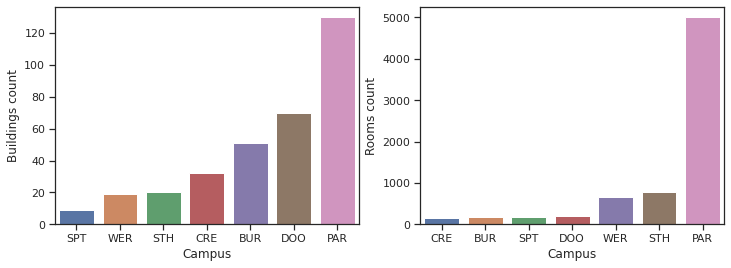
\includegraphics[width=12cm,keepaspectratio=true]{snap-1}
\caption{Distribution of buildings and rooms across campuses}
\label{fig:expo-image-1}
\end{figure}

Using room category data and merging it with space metadata, we were able to figure out the distribution of meeting rooms and toilet facilities across buildings in the Parkville campus as shown in Figure \ref{fig:expo-image-2}. We saw that \texttt{333 Exhibition st} buildings have the highest number of meeting rooms and \texttt{The spot} building has the highest number of toilet facilities.

\begin{figure}[H]
\centering
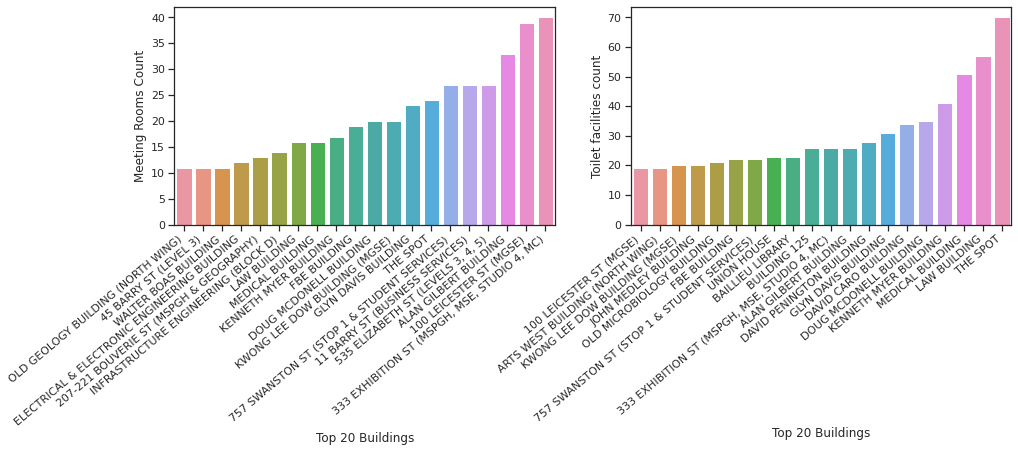
\includegraphics[width=16cm,keepaspectratio=true]{snap-2}
\caption{Distribution of meeting rooms and toilet facilities across buildings in Parkville Campus}
\label{fig:expo-image-2}
\end{figure}

\subsubsection{Supply-demand Analysis}

After exploring different properties and aspects of the data, we tried to see and understand how data can be used to get the basic intuition of the problem by performing supply-demand analysis across buildings on different campuses.

\paragraph{Parkville Campus}

We created several supply-demand plots across various covariates which helped to see the need for space optimization in the Parkville Campus. Initially, we created supply-demand plots based on the very trivial preference of staff members trying to book a meeting room in the same building where they are located. This plot is shown in Figure \ref{fig:expo-image-3}. As per the plot, we can see space optimization problems in terms of supply and demand proportion especially in the \texttt{Law Building}, \texttt{Doug Mcdonell building}, and \texttt{Kenneth Myer building}.

\begin{figure}[H]
\centering
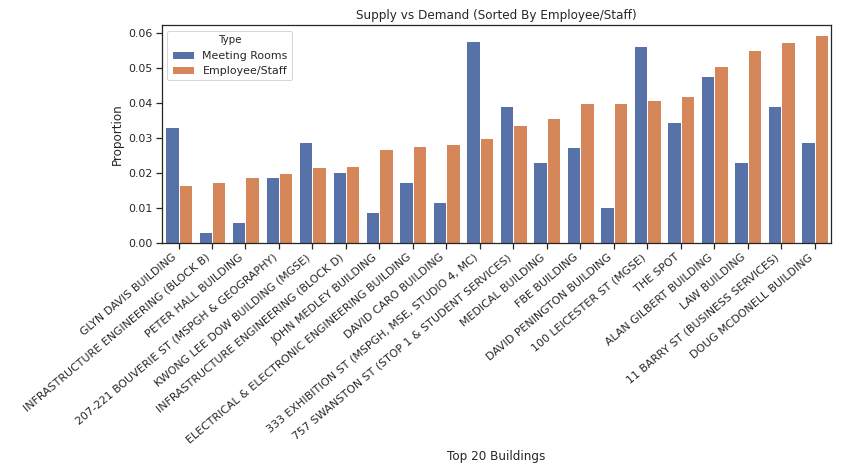
\includegraphics[width=10cm,keepaspectratio=true]{snap-3}
\caption{Supply vs Demand of meeting rooms across buildings in Parkville Campus}
\label{fig:expo-image-3}
\end{figure}

 Similarly, we created a supply-demand plot on the same trivial preference of students trying to access a toilet facility in the same building which is shown in Figure \ref{fig:expo-image-4}. Again, we can see that the space optimization problem in terms of supply and demand proportion, especially for \texttt{Redmond barry building}.
 
\begin{figure}[H]
\centering
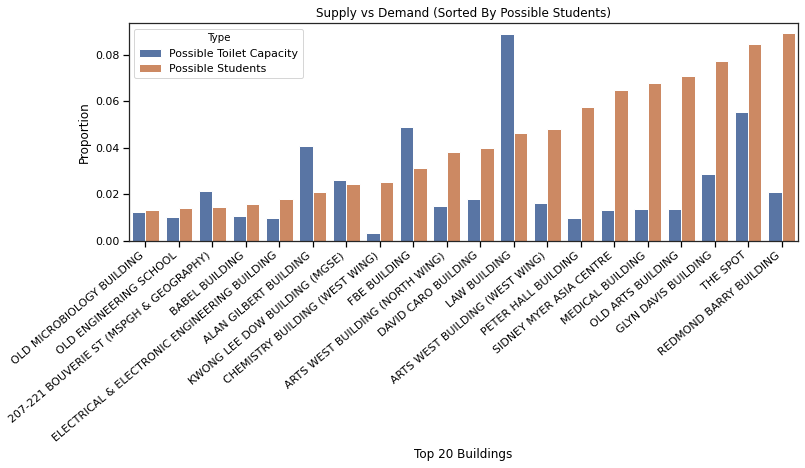
\includegraphics[width=10cm,keepaspectratio=true]{snap-4}
\caption{Supply vs Demand of toilet facilities across buildings in Parkville Campus}
\label{fig:expo-image-4}
\end{figure}

We have explored several other covariates or factors concerning supply-demand in Section \ref{factor_analysis} which will eventually help us to perform space optimization on the underlying problem.

\paragraph{Other Campuses}

We extended our analysis of supply-demand to campuses other than Parkville in order to get more ideas about the space optimization problem. We used the absolute supply-demand proportion for the meeting room's capacity with respect to the demand and created plot for different campuses as shown in the Figure \ref{fig:sp-others-1}. The results can be summarized as follows.

\begin{itemize}
    % \item \textbf{Burnley Campus:} Due to the lack of meeting rooms data, we were not able to do supply-demand analysis for this campus. We were not able to find any rooms which can be considered as meeting rooms in this campus which shows the importance of data as the primary requirement for better analysis.
    
    \item \textbf{Southbank Campus:} As per the Southbank plot, we can clearly highlight the supply-demand problem with respect to the meeting rooms, especially for the \texttt{Elisabeth Murdoch Building}. This campus seems to have a high number of supply-demand imbalance as mostly all of the buildings for which data was provided seems to have space optimization issue as seen from the Figure \ref{fig:sp-others-1}.
    
    \item \textbf{Werribee Campus:} As per the Werribee plot, we can clearly identify a major space optimization problem in terms of supply-demand of meeting rooms in \texttt{Werribee Pathology Building} as per the provided data. We can also see that the other buildings seem to have an adequate proportion of supply to balance the demand.
    
    \item \textbf{Creswick Campus:} We were able to find 3 buildings which provided both supply-demand data for meeting rooms analysis. As per the plot, we can see that the demand in \texttt{Creswick Research Laboratories} is high as compared to the supply of the meeting rooms where other buildings seem to have an adequate supply.
    
    \item \textbf{Shepparton Campus:} We couldn't find much supply-demand data in terms of meeting rooms for this campus. As per the Shepparton plot, we could only find 1 building for which we have adequate supply-demand data and the \texttt{49 Graham St, Shepparton} building seems to have a supply-demand problem as the proportion for the demand of meeting rooms is higher than the supply.
    
    % \item \textbf{Dookie Campus:} Due to the lack of meeting rooms data, we were not able to do supply-demand analysis for this campus. We were not able to find any rooms which can be considered as meeting rooms in this campus which shows the importance of data as the primary requirement for better analysis.
    
\end{itemize}

\begin{figure}[H]
\centering
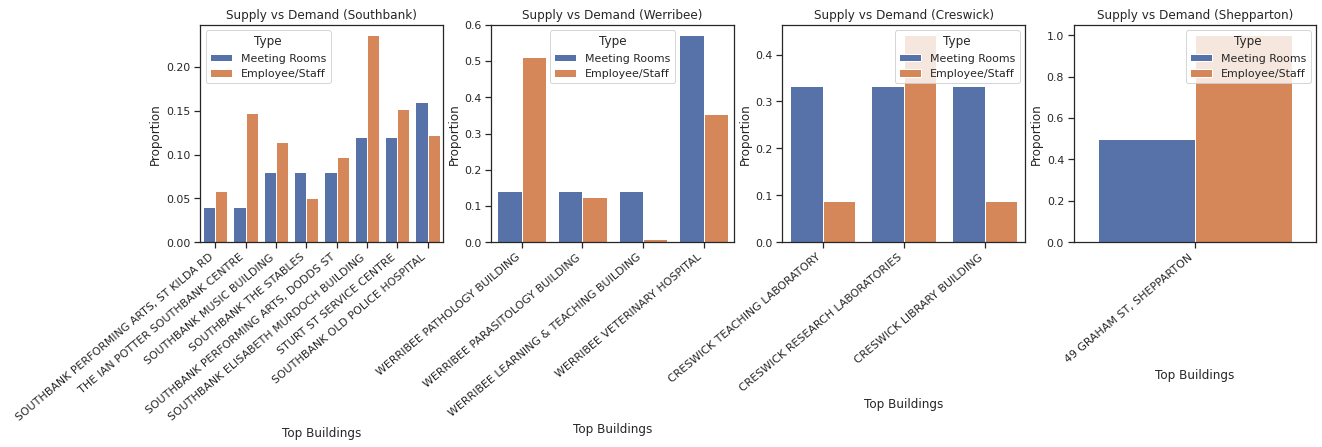
\includegraphics[width=17cm,keepaspectratio=true]{supply_demand_others_mr}
\caption{Supply vs Demand of meeting rooms across buildings in different campuses}
\label{fig:sp-others-1}
\end{figure}

Similarly, we used the absolute supply-demand proportion for the toilet facilities capacity with respect to the demand and created a plot for different campuses as shown in the Figure \ref{fig:sp-others-2}. The results can be summarized as follows.

\begin{itemize}
    % \item \textbf{Burnley Campus:} Due to the lack of toilet facilities data, we were not able to do supply-demand analysis for this campus. We were not able to find any buildings for which data is provided for both supply and demand, which shows the importance of data as the primary requirement for better analysis.
    
    \item \textbf{Southbank Campus:} As per the Southbank plot, we can clearly highlight the supply-demand problem with respect to the toilet facilities, especially for the \texttt{Ian Potter Southbank Centre}. This is followed by \texttt{Southbank Music Building} and \texttt{Southbank Art Studios 1}. Other buildings inside the campus seem to have a good supply-demand balance in terms of students attending classes and provided toilet facilities.
    
    \item \textbf{Werribee Campus:} As per the Werribee plot, we can clearly identify a major space optimization problem in terms of supply-demand of toilet facilities in \texttt{Werribee Learning \& Teaching Building} as per the provided data. We couldn't find supply-demand data for more buildings on this campus in terms of toilet facilities and student classes.
    
    \item \textbf{Creswick Campus:} We were able to find only 1 building which provided both supply-demand data for toilet facilities analysis. As per the plot, we can clearly see that the demand in the \texttt{Creswick Seminar  Centre} is high as compared to the supply of the toilet facilities. We couldn't find supply-demand data for more buildings on this campus in terms of toilet facilities and student classes.
    
    \item \textbf{Shepparton Campus:} We couldn't find much supply-demand data in terms of toilet facilities for this campus. As per the Shepparton plot, \texttt{Dookie-Swinburne Hall} building seems to have a supply-demand problem as the proportion for the demand for toilet facilities is higher than the supply.
    
    % \item \textbf{Dookie Campus:} Due to the lack of toilet facilities data, we were not able to do supply-demand analysis for this campus. We were not able to find any buildings for which data is provided for both supply and demand, which shows the importance of data as the primary requirement for better analysis.
    
\end{itemize}



\begin{figure}[H]
\centering
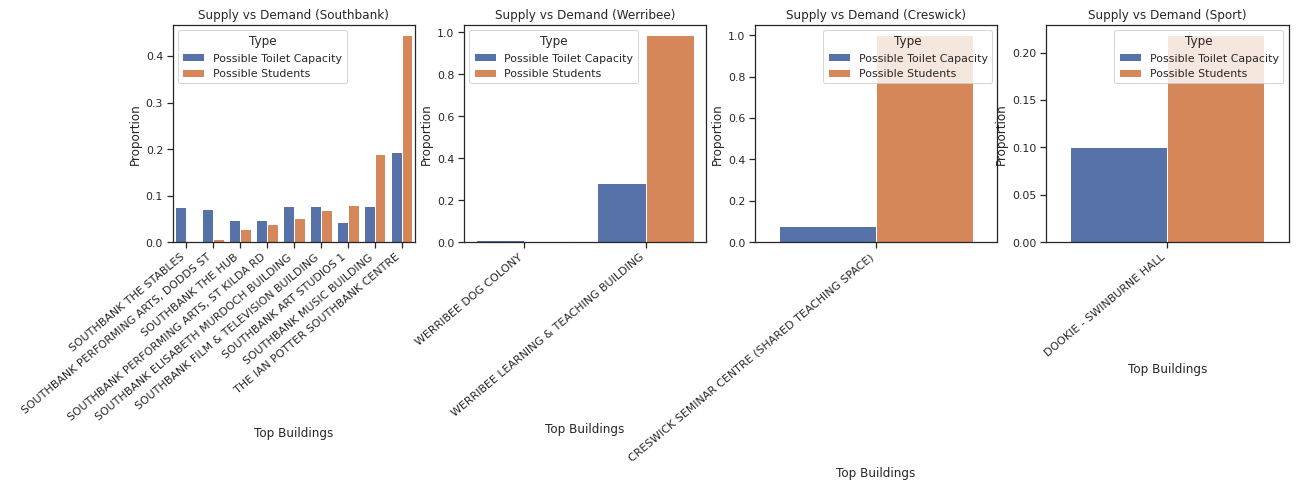
\includegraphics[width=17cm,keepaspectratio=true]{supply_demand_others_tr}
\caption{Supply vs Demand of toilet facilities across buildings in different campuses}
\label{fig:sp-others-2}
\end{figure}


\subsection{Factors Analysis} \label{factor_analysis}

In this section, we will explore different preferences or factors that concern the effect of booking a meeting room or using a toilet facility. These factors directly impact the expected reward from a building or floor, thereby used extensively in solving the same problem from different situations.

\subsubsection{Factors for booking a meeting room}
In this section, we will look at different factors that can impact the probability of booking a meeting room.

\begin{enumerate}
    \item \textbf{Same Building}: Using this factor, the employee wants to book a meeting room in the same building. This is a default factor that is considered automatically while solving our optimization problem of finding the nearest building from a particular building.
    
    \item \textbf{Same Floor}: Using this factor, the employee wants to book a meeting room on the same floor in a particular building. Again, this is a default factor that is considered automatically while solving our optimization problem of finding the nearest floor from a particular floor.
    
    \item \textbf{COVID-19 Lockdown Situation}: Using this factor, an employee can express the COVID-19 lockdown scenario which can directly impact the expected rewards gained from the targeted buildings or floors. This factor can be used to represent \texttt{Strict Lockdown} condition which means there is no demand at all, \texttt{Medium Lockdown} condition which means there is 25\% demand, and \texttt{Low Lockdown} condition which means there is 50\% demand.
    
    \item \textbf{High Capacity:} Using this factor, an employee can target the situation of booking a meeting room with high capacity. This can be inferred using the average room size provided by the data for each meeting room.
    
    \item \textbf{Required Capacity(C):} Using this factor, an employee can target the situation of booking a meeting room with a very specific capacity requirement $C$. This can be inferred using the supply of room capacity provided by the data for each meeting room.
    
    \item \textbf{With Equipment:} Using this factor, an employee can express the requirement of booking a meeting room with useful equipment. This can be inferred using the \texttt{av-equipment} dataset that helps us to understand the equipment capacity distribution across different buildings and floors.
    
    \item \textbf{Room Conditions:} Using this factor, employee can express the requirement of booking a meeting room with \texttt{Excellent}, \texttt{Very Good} or \texttt{Good} condition. This can be inferred using the room condition property provided in the space dataset.
    
    \item \textbf{Easy Availability}: Using this factor, an employee wants to book a meeting room that is easily available which can be inferred using meeting room usage data. \textbf{Stop 1} has the most number of excellent rooms based on the usage data and out of all the meeting rooms, only 3\% can be booked. Buildings with low demand have low usage of the meeting rooms as shown in Figure \ref{usagedata}.
    
\begin{figure}[H]
    \centering
    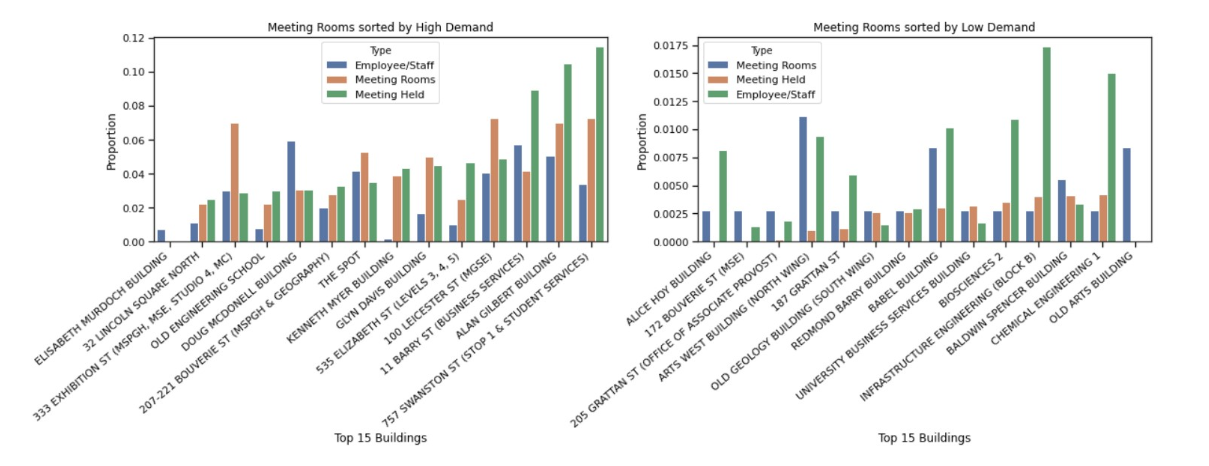
\includegraphics[width=1\textwidth]{resources/images/snap5.PNG}
    \caption{Supply vs demand analysis for easy availability factor}
    \label{usagedata}
\end{figure}

\end{enumerate}

\subsubsection{Factors for using a toilet facility}

In this section, we will look at different factors that can impact the probability of using a toilet facility.

\begin{enumerate}
    \item \textbf{Same Building}: Using this factor, a student wants to use a toilet facility in the same building. This is a default factor that is considered automatically while solving our optimization problem of finding the nearest building from a particular building.
    
     \item \textbf{Same Floor}: Using this factor, a student wants to use a toilet facility on the same floor in a particular building. Again, this is a default factor that is considered automatically while solving our optimization problem of finding the nearest floor from a particular floor.
     
     \item \textbf{COVID-19 Lockdown Situation}: Using this factor, a student can express the COVID-19 lockdown scenario which can directly impact the expected rewards gained from the targeted buildings or floors. This factor can be used to represent \texttt{Strict Lockdown} condition which means there is no demand at all, \texttt{Medium Lockdown} condition which means there is 25\% demand, and \texttt{Low Lockdown} condition which means there is 50\% demand.
    
    \item \textbf{High Capacity:} Using this factor, the situation can be targeted using a toilet facility with high capacity. This can be inferred using the average room size provided by the data for each toilet room.
    
    \item \textbf{Required Capacity(C):} Using this factor, the situation can be targeted at using a toilet facility with a very specific capacity requirement $C$. This can be inferred using the supply of room capacity provided by the data for each toilet room.
    
    \item \textbf{Easy Availability}: Using this factor, a student wants to use a toilet facility which is easily available that can be inferred using the average duration of classes in a building or a particular floor. If classes have a longer duration in a building or floor, then that building should have facilities with better capacity as availability will be less. As per our analysis, it can be seen that the Old Physics building has a very long duration of lectures but it has 1\% of the total capacity of toilets.
    
    \item \textbf{Room Conditions}: Using this factor, student can express the requirement of using a toilet facility with \texttt{Excellent}, \texttt{Very Good} or \texttt{Good} condition. This can be inferred using the room condition property provided in the space dataset. Students usually prefer accessing the toilet facilities which are in good condition and in the same building where their respective classes are conducted. We can observe this correlation with supply-demand as shown in Figure \ref{toilet}.
    
    \begin{figure}[H]
    \centering
    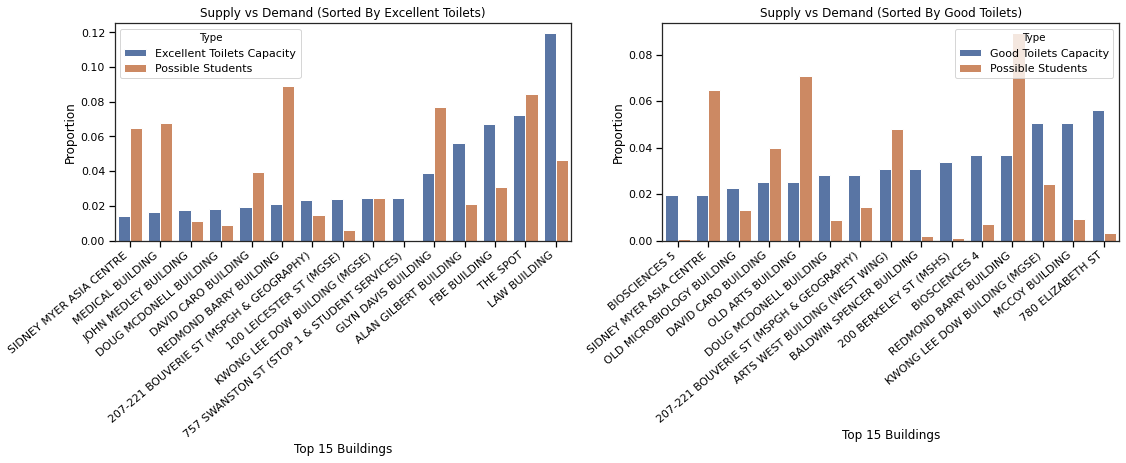
\includegraphics[width=15cm]{resources/images/snap-10.png}
    \caption{Supply vs demand analysis with toilet room conditions factor}
    \label{toilet}
\end{figure}

    
\end{enumerate}
